\begin{figure}[htbp]
\section*{ GLI3}
\centering
\begin{subfigure}[b]{0.95\textwidth}
\centering
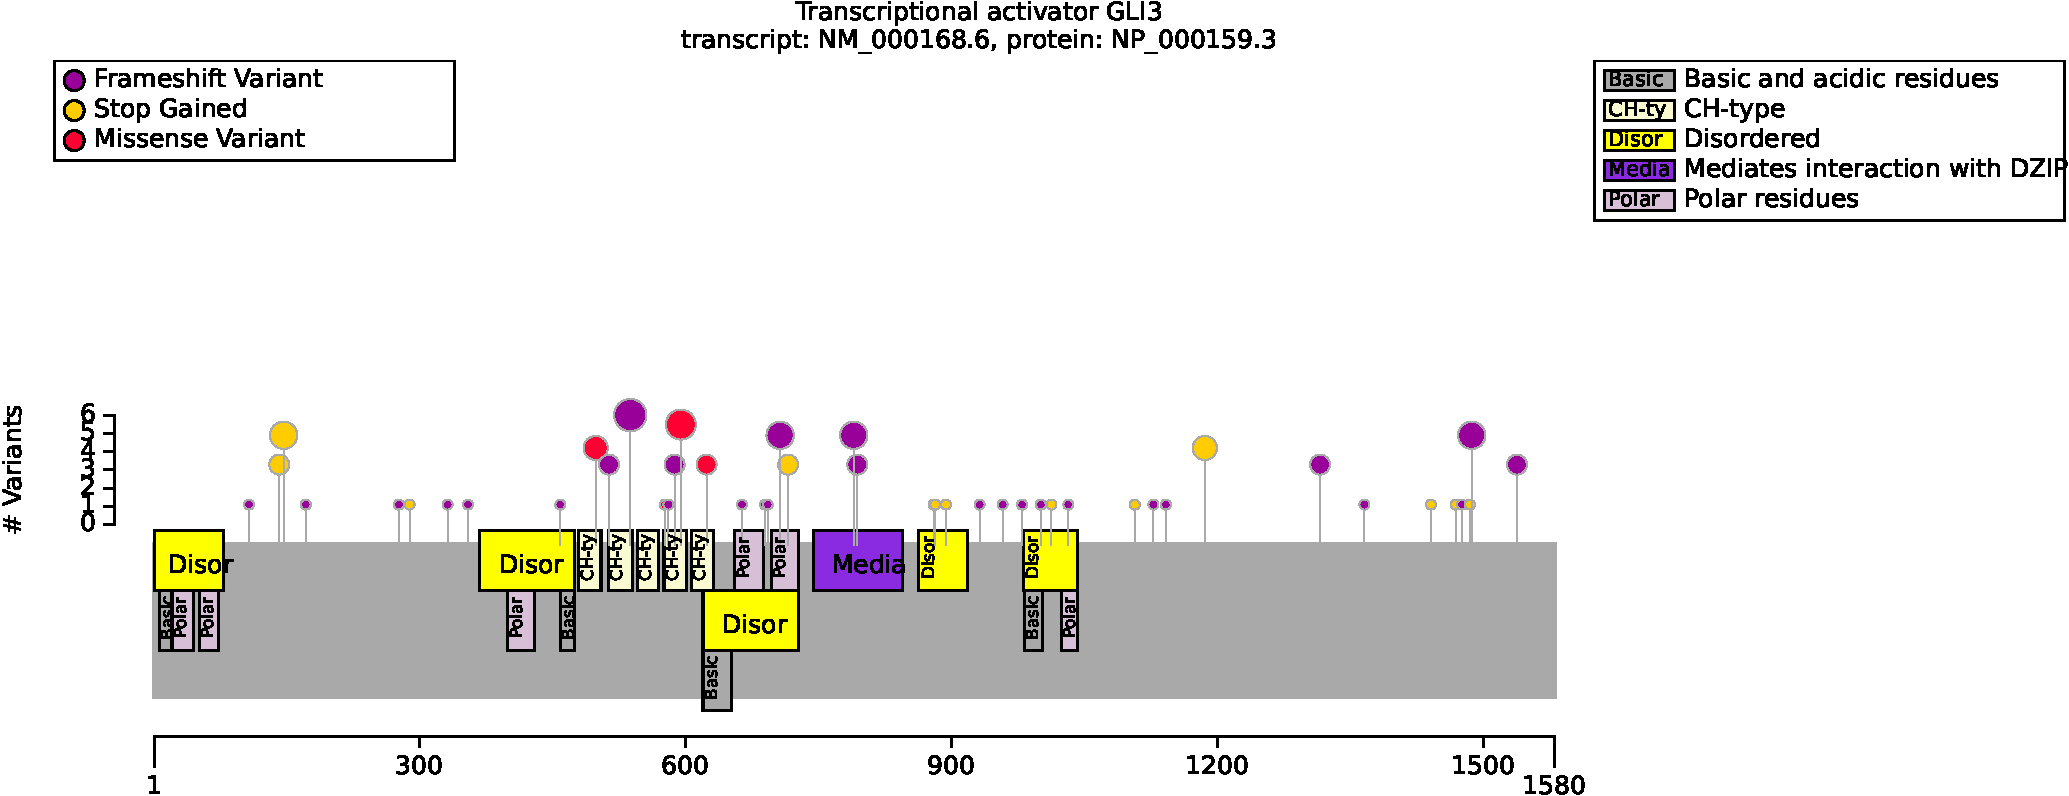
\includegraphics[width=\textwidth]{ img/GLI3_protein_diagram.pdf} 
\captionsetup{justification=raggedright,singlelinecheck=false}
\caption{Distribution of variants in GLI3}
\end{subfigure}

\vspace{0.4em}

\begin{subfigure}[b]{0.95\textwidth}
\centering
\resizebox{\textwidth}{!}{
\begin{tabular}{llllrr}
\toprule
HPO term & Fs in mid region or splice & other & p-value & adj. p-value\\
\midrule
Preaxial foot polydactyly [HP:0001841] & 5/25 (20\%) & 32/57 (56\%) & 0.003 & 0.021\\
Y-shaped metacarpals [HP:0006042] & 11/23 (48\%) & 4/56 (7\%) & $9.94\times 10^{-5}$ & 0.001\\
Y-shaped metatarsals [HP:0010567] & 11/19 (58\%) & 4/50 (8\%) & $3.25\times 10^{-5}$ & $7.80\times 10^{-4}$\\
Nail dysplasia [HP:0002164] & 7/20 (35\%) & 2/54 (4\%) & 0.001 & 0.009\\
Anal atresia [HP:0002023] & 7/25 (28\%) & 3/57 (5\%) & 0.007 & 0.036\\
\bottomrule
\end{tabular}
}
\captionsetup{justification=raggedright,singlelinecheck=false}
\caption{Fisher Exact Test performed to compare HPO annotation frequency with respect to Fs in mid region or splice and other. Total of
        24 tests were performed. }
\end{subfigure}
\vspace{0.4em}
\begin{subfigure}[b]{0.95\textwidth}
\centering
\resizebox{\textwidth}{!}{
\begin{tabular}{llllrr}
\toprule
HPO term & Truncating variants in Exon 15 & other & p-value & adj. p-value\\
\midrule
Macrocephaly [HP:0000256] & 13/16 (81\%) & 15/42 (36\%) & 0.003 & 0.017\\
Preaxial foot polydactyly [HP:0001841] & 7/28 (25\%) & 30/54 (56\%) & 0.010 & 0.050\\
Syndactyly [HP:0001159] & 5/17 (29\%) & 33/38 (87\%) & $4.82\times 10^{-5}$ & 0.001\\
Postaxial foot polydactyly [HP:0001830] & 9/20 (45\%) & 2/35 (6\%) & $8.91\times 10^{-4}$ & 0.011\\
Anal atresia [HP:0002023] & 8/28 (29\%) & 2/54 (4\%) & 0.002 & 0.017\\
\bottomrule
\end{tabular}
}
\captionsetup{justification=raggedright,singlelinecheck=false}
\caption{Fisher Exact Test performed to compare HPO annotation frequency with respect to Truncating variants in Exon 15 and other. Total of
        24 tests were performed. }
\end{subfigure}
\vspace{0.4em}
\begin{subfigure}[b]{0.95\textwidth}
\centering
\resizebox{\textwidth}{!}{
\begin{tabular}{llllrr}
\toprule
HPO term & Variants in C-terminal third & other & p-value & adj. p-value\\
\midrule
Macrocephaly [HP:0000256] & 13/15 (87\%) & 15/43 (35\%) & $7.31\times 10^{-4}$ & 0.004\\
Postaxial hand polydactyly [HP:0001162] & 15/16 (94\%) & 21/49 (43\%) & $3.40\times 10^{-4}$ & 0.003\\
Syndactyly [HP:0001159] & 5/16 (31\%) & 33/39 (85\%) & $2.25\times 10^{-4}$ & 0.003\\
Postaxial foot polydactyly [HP:0001830] & 9/16 (56\%) & 2/39 (5\%) & $7.35\times 10^{-5}$ & 0.002\\
\bottomrule
\end{tabular}
}
\captionsetup{justification=raggedright,singlelinecheck=false}
\caption{         Fisher Exact Test performed to compare HPO annotation frequency with respect to Variants in C-terminal third and other. Total of
        24 tests were performed. }
\end{subfigure}
\vspace{0.4em}
\caption{ The cohort comprised 82 individuals (3 females, 7 males, 72 with unknown sex). A total of 34 HPO terms were used to annotate the cohort. Disease diagnoses: Greig cephalopolysyndactyly syndrome (OMIM:175700) (51 individuals), Pallister-Hall syndrome (OMIM:146510) (21 individuals), Polydactyly, postaxial, types A1 and B (OMIM:174200) (10 individuals). Genotype-Phenotype-Correlations in GLI3 have been extensive investigated, with findings being similar 
but not identical to those reported here \cite{PMID_15739154,PMID_22903559,PMID_33058447,PMID_24736735,PMID_9354780,PMID_28224613,PMID_34482537}. A total of 49 unique variant alleles were found in \textit{GLI3} (transcript: \texttt{NM\_000168.6}, protein id: \texttt{NP\_000159.3}).}
\end{figure}
